\documentclass[12pt, a4paper, oneside]{book}

%---------------------------------------------------------   
\usepackage[english,romanian,magyar]{babel}       
\usepackage[utf8]{inputenc}
\usepackage[a4,center,axes]{crop}
\usepackage{calc}
\usepackage{t1enc}
\usepackage{amsthm}
\usepackage{rotating}
\usepackage{amssymb}
\usepackage{lscape}
\usepackage{anysize}
\usepackage{setspace} 
\usepackage{comment}
\usepackage{graphicx}
\usepackage{setspace} 
\usepackage{tocloft}
\usepackage{indentfirst}
\usepackage{url}
\usepackage[top=3cm, bottom=2cm, left=3cm, right=2cm]{geometry}

%---------------------------------------------------------
%%
%%
%% alapformázások
%%
%%
\sloppy                        % sorkizárás kezelése
\clubpenalty = 10000           % árvasorok
\widowpenalty = 10000          % fatyúsorok
\raggedbottom                  % függõleges kizárás az oldalon
\setcounter{secnumdepth}{3}    % alcimek számozási mélysége
\setcounter{tocdepth}{3}       % tartalomjegyzék mélysége
\brokenpenalty = 10000         % lap aljai elválasztások tiltása
\doublehyphendemerits = 80000  % egymást követõ elválasztások

%\marginsize{2cm}{2cm}{2cm}{2cm} %marók beállítása
\onehalfspacing %sorközök megaddása

\theoremstyle{tetel}
\newtheorem{mydef}{értelmezés}[chapter]
\newtheorem{megj}{megjegyzés}[chapter]

\def\partro#1{\foreignlanguage{romanian}{\addcontentsline{tro}{part}{%\if@mainmatter\protect\numberline{\thechapter.}\fi
\MakeUppercase{#1}}}}
\def\chapterro#1{\foreignlanguage{romanian}{\addcontentsline{tro}{chapter}{\if@mainmatter\protect\numberline{\thechapter.}\fi#1}}}
\def\sectionro#1{\foreignlanguage{romanian}{\addcontentsline{tro}{section}{\protect\numberline{\thesection.}#1}}}
\def\subsectionro#1{\foreignlanguage{romanian}{\addcontentsline{tro}{subsection}{\protect\numberline{\thesubsection.}#1}}}
\def\subsubsectionro#1{\foreignlanguage{romanian}{\addcontentsline{tro}{subsubsection}{\protect\numberline{\thesubsubsection.}#1}}}

%roman tartalom def
%---------------------------------------------------------
\newcommand{\nombreindice}{Cuprins}
\newlistof{indice}{tce}{\nombreindice}

\newcommand\capterro[1]{%
  \addcontentsline{tce}{chapter}{\protect\makebox[1.3em][l]{\thechapter.}#1}}
\newcommand\secro[1]{%
  \addcontentsline{tce}{section}{\protect\makebox[2.8em][l]{\thesection.}#1}}
\newcommand\ssecro[1]{%
\addcontentsline{tce}{subsection}{\protect\makebox[3em][l]{\thesubsection.}#1}}

%angol tartalom def
%---------------------------------------------------------

\newcommand{\tcontents}{Table Of Contents}
\newlistof{indiceen}{tcen}{\tcontents}

\newcommand\capteren[1]{%
  \addcontentsline{tcen}{chapter}{\protect\makebox[1.3em][l]{\thechapter.}#1}}
\newcommand\secen[1]{%
  \addcontentsline{tcen}{section}{\protect\makebox[2.8em][l]{\thesection.}#1}}
\newcommand\ssecen[1]{%
\addcontentsline{tcen}{subsection}{\protect\makebox[3em][l]{\thesubsection.}#1}}

%---------------------------------------------------------
\newcommand*{\field}[1]{\mathbb{#1}}

%---------------------------------------------------------

%---------------------------------------------------------
\begin{document}
\pagenumbering{arabic}

%magyar borito
%--------------------------------------------------------
\newpage
\thispagestyle{empty}
\begin{center}
    \Large SAPIENTIA ERDÉLYI MAGYAR TUDOMÁNYEGYETEM\\
    \Large MŰSZAKI ÉS HUMÁNTUDOMÁNYOK KAR, MAROSVÁSÁRHELY\\
    \Large SZOFTVERFEJLESZTÉS SZAK\\
\end{center}

\begin{center}
 	\vspace{2cm}\LARGE \textbf{DeepArt}\\
	 \vspace{1cm}\LARGE \textbf{MESTERI DISSZERTÁCIÓ}\\
\end{center}

\vspace{2cm}
\begin{figure}[htb]
\hspace{5.7cm}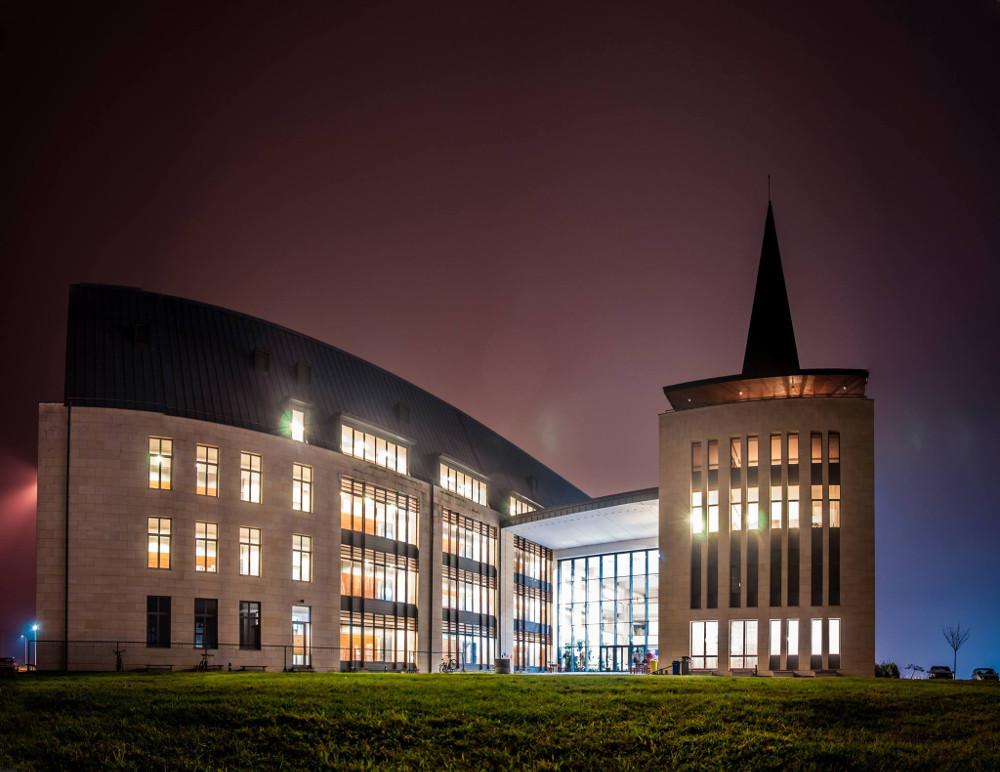
\includegraphics[bb = 0 0 160 160]{sapi.jpg}
\end{figure}

\vspace{2cm}
\begin{center}
\begin{tabular}{lcccccccccccl}
    TÉMAVEZETŐ:&&&&&&& &&&&&SZERZŐ:\\
     dr. Iclănzan Dávid&&&&&& &&&&&&Szilágyi Ervin\\
	Egyetemi tanár
\end{tabular}
\end{center}

\begin{center}
    \vspace{0.5cm}\textbf{2017 Június}
\end{center}
\vspace*{\fill}
%roman borito
%-------------------------------------------------------------
\newpage
\thispagestyle{empty}
\begin{center}
    %\Large UNIVERSITATEA BABE\c{S}-BOLYAI CLUJ-NAPOCA\\
    \Large UNIVERSITATEA SAPIENTIA TÂRGU-MURE\c{S}\\
    \Large FACULTATEA DE \c{S}TIIN\c{T}E TEHNICE \c{S}I UMANISTE\\
    \Large SPECIALIZAREA DEZVOLTARE DE SOFTWARE\\
\end{center}

\begin{center}
    \vspace{3cm}\LARGE \textbf{DeepArt}\\
    \vspace{1cm}\LARGE\textbf{Lucrare de master}\\
\end{center}

\vspace{2cm}
\begin{figure}[htb]
\hspace{5.7cm}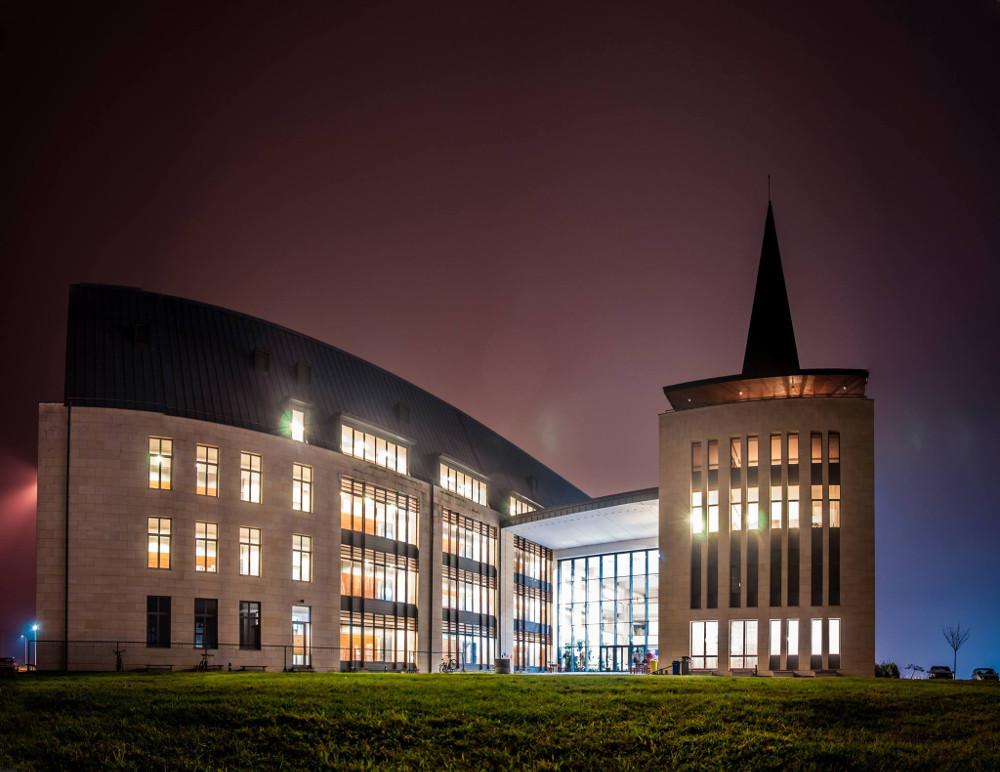
\includegraphics[bb = 0 0 160 160]{sapi.jpg}
\end{figure}

\vspace{2cm}
\begin{center}
\begin{tabular}{lcccccccccccl}
    Coordonator \c{s}tiin\c{t}ific:&&&&&&& &&&&&Absolvent:\\
     dr. Iclănzan Dávid&&&&&& &&&&&&Szilágyi Ervin\\

\end{tabular}
\end{center}

\begin{center}
    \vspace{1cm}\textbf{2017 Iunie}
\end{center}

%angol borito
%-------------------------------------------------------------

\newpage
\thispagestyle{empty}
\begin{center}
    %\Large BABE\c{S}-BOLYAI UNIVERSITY CLUJ-NAPOCA\\
    \Large SAPIENTIA UNIVERSITY TÂRGU MURE\c{S}\\
    \Large FACULTY OF TECHNICAL AND HUMAN SCIENCES\\
    \Large SOFTWARE DEVELOPMENT SPECIALIZATION\\
\end{center}

\begin{center}
    \vspace{3cm}\LARGE \textbf{DeepArt}\\
    \vspace{1cm}\LARGE \textbf{Master Thesis}\\
\end{center}

\vspace{2cm}
\begin{figure}[htb]
\hspace{5.7cm}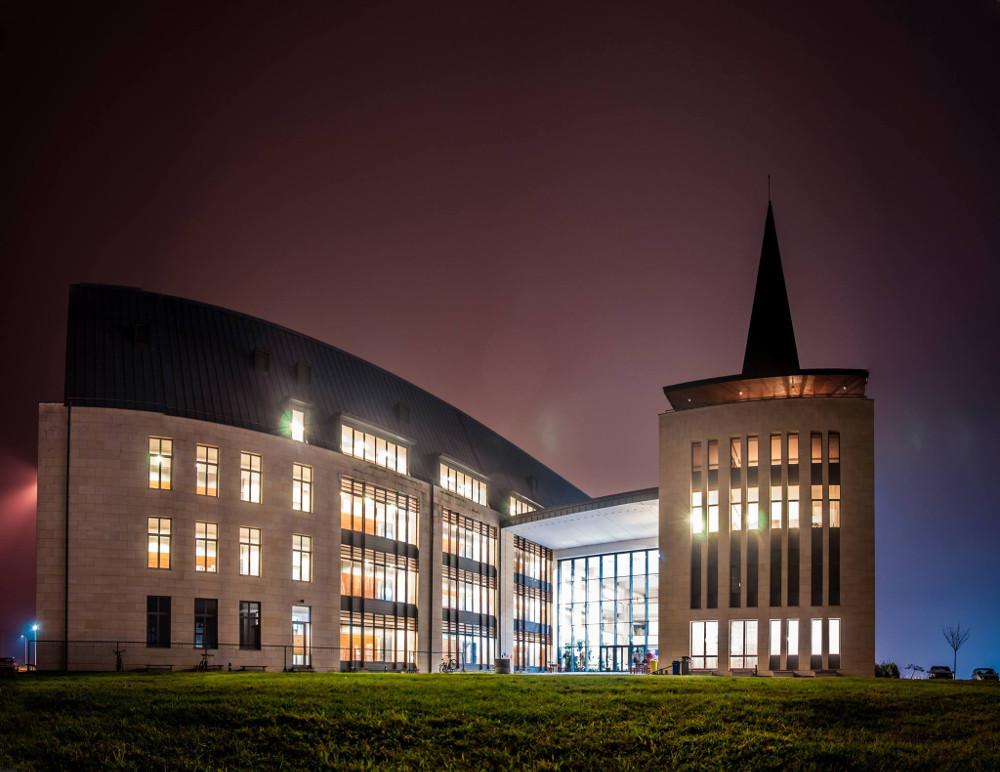
\includegraphics[bb = 0 0 160 160]{sapi.jpg}
\end{figure}

\vspace{2cm}
\begin{center}
\begin{tabular}{lcccccccccccl}
     Advisor: & & &&&& &&&&&& Student:\\
     dr. Iclănzan Dávid &&&&&& &&&&&& Szilágyi Ervin\\
\end{tabular}
\end{center}

\begin{center}
    \vspace{1cm}\textbf{2017 June}
\end{center}

%eredetisegi nyilatkozat
%-------------------------------------------------------------
\newpage
\thispagestyle{empty}
eredetisegi nyilatkozat
%kivonat magyar
%-------------------------------------------------------------
\newpage
\thispagestyle{empty}
\begin{center}
    \Large KIVONAT
\end{center}

kivonat

\begin{flushright}
\textbf{Szilagyi Ervin,}\\
.........................
\end{flushright}

%kivonat roman
%-------------------------------------------------------------
\newpage
\thispagestyle{empty}
\begin{center}
    \Large ABSTRACT
\end{center}

abstract

\begin{flushright}
\textbf{Szilagyi Ervin,}\\
.........................
\end{flushright}

%kivonat angol
%-------------------------------------------------------------
\newpage
\thispagestyle{empty}
\begin{center}
    \Large ABSTRACT
\end{center}

english abstract


\begin{flushright}
\textbf{Szilagyi Ervin,}\\
.........................
\end{flushright}

%tartalom jegyzek
%-------------------------------------------------------------
\newpage
\tableofcontents
\newpage
\listofindice
\newpage
\listofindiceen

\selectlanguage{magyar}

%-------------------------------------------------------------
\chapter{Bevezető}
\capterro{Întroducere}
\capteren{Indroduction}

Napjainkban a képfeldolgozás egy eléggé elterjedt kutatási terület. A kutatások célja főleg az információ kinyerésére, gépi látás kivitelézésére irányult. Minderre kiváló megoldást jelentett a deep konvolúciós hálok (ConvNets)\cite{1}\cite{2} sikeres használata növelve ezzel ezek népszerűségét. Fontos megjegyezni, hogy a konvolúciós neuron hálok felfedezése már pár évtizede történt, tehát maga a technológia már régebb ismert volt. Az újrafelfedezésüket és hirtelen népszerűség növekedését annak köszönhetik, hogy az utóbbi években olyan hardveres megoldások jelentek meg amik lehetővé teszik az ilyen típusú hálok létrehozását és működtetését. 
\newline 
\indent
Az Nvidia cég 2007-ben bevezette az Nvidia CUDA platformot\cite{3}. Ez egy komoly, használható fejlesztőkörnyezetett jelentett olyan fejlesztők számára akik nagy méretű adatpárhuzamos algoritmusokat szerettek volna fejleszteni. A CUDA környezet direkt elérhetőséget nyújt a videókártya utasításkészletéhez megengedve ezzel ennek a programozását. Ugyanakkor számos olyan videókártya került piacra ami egyre komolyabb számítási készségekkel bírt. Ezt a lehetőséget értelemszerűen a kutatók ki is használták így számos újabb publikáció és javaslat jelent meg amik neuron hálókat használnak az illető probléma megoldására.
\newline
\indent
A deep konvolúciós hálok népszerűségének növekedésével egyre több olyan fejlesztői környezet jelent meg amiknek célja a mesterséges intelligencia feladatok megoldása. Ilyen könyvtárak például a Caffe\cite{4}, Keras\cite{5}, Theano\cite{6}, Tensorflow\cite{7}, Torch\cite{8} stb. Ezek a környezetekben, habár különböző stílusban de egyazon problémákra hivatottak gyors és egyszerű megoldásokat ajánla ugyanúgy mezei szoftverfejlesztők, mint kutatók számára.
\newline
\indent
Az gépi látás egyik fontos alkalmazási területe a képen levő tárgyak, élőlények emberek felismerése. Ilyen területen a konvolúciós hálok kimagasló teljesítményt nyújtanak, olyannyira, hogy egyes kisérletek szerint ez már nemhogy az emberi látással megegyező, hanem azt felülmúló teljesítméynt nyújtanak\cite{9}. Feltevődik a kérdés, hogyha ennyire szofisztikált a gépi látás, akkor nem-e lehetne használni arra, hogy új képeket alkosson. Amint kiderült erre is alkalmasak. Az általam bemutandó dolgozat is ezt a témát próbálja megcélozni. A gépi látás a tárgyak, élőlények mellett képes felismerni maga a kép művészeti stílusát. Ez elsősorban kihasználható arra, hogy híres művészek alkotásait csoportosítsuk, rendszerezzül\cite{10}, de amint e dolgozatból ki fog derülni, ki lehet használni arra is, hogy egy művészeti stílust egy adott festményről átvigyük egy mindennapi képre, fotóra. 
\newline
\indent
A dolgozatom célja magyar híres festőművészek festészeti stílusát átvenni és ezt alkalmazni midennapi képekre illetve mozgóképekre. Eddigiekben, ahhoz hogy egy mindennapi fényképből művészeti képet varázsoljunk, képszerkesztő szoftverek segítségével lehetett elérni manuálisan. Mindezt egy olyan egyén végezhette, akinek képszerkesztési illetve képmanipulálási szakismere volt adott képszerkesztési szoftverkörnyezetben. Magatól értődik az, hogy ez mozgóképek esetében egy időigényes folyamat. Dolgozatom mindezekre megoldást próbál adni, azáltal, hogy az általam elkészített szoftvert bárki használhatja, nincs szükség különböző képszerkesztői szakértelemre, emellett a folyamat ideje jelentősen csökkenni fog. 

%-------------------------------------------------------------
\chapter{Hasonló rendszerek feltérképezése}
\capterro{Studiu bibliografic}
\capteren{Bibliographic study}

bib study



%-------------------------------------------------------------
\chapter{A rendszer}
\capterro{Sistemul}
\capteren{The system}

%-------------------------------------------------------------
\section{Áttekintés}
\secro{Privire de ansamblu asupra}
\secen{Overview}

a rendszer

%----------------------------------------------------------------
\chapter{Összefoglaló}
\capterro{Concluzie}
\capteren{Conclusion}

összefoglaló

% Ábrajegyzék
%---------------------------------
\newpage
 \listoffigures


% thebibliography
%---------------------------------
\newpage
\begin{thebibliography}{1}

\bibitem {1}
Krizhevsky, A., Sutskever, I., and Hinton, G. E. ImageNet classification with deep convolutional neural networks (2012)

\bibitem{2}
Zeiler, M. D. and Fergus, R. Visualizing and understanding convolutional networks (2013)

\bibitem{3}
\url {https://en.wikipedia.org/wiki/CUDA} (2017.04.24)

\bibitem{4}
\url {http://caffe.berkeleyvision.org} (2017.04.24)

\bibitem{5}
\url {https://keras.io/} (2017.04.24)

\bibitem{6}
\url {http://deeplearning.net/software/theano/} (2017.04.24)

\bibitem{7}
\url {https://www.tensorflow.org/} (2017.04.24)

\bibitem{8}
\url {http://torch.ch/} (2017.04.24)

\bibitem{9}
\url {https://computerstories.net/microsoft-computer-outperforms-human-image-recognition-12028} (2017.04.29)

\bibitem{10}
Kevin Alfianto, Mei-Chen Yeh, Kai-Lung Hua - Artist-based Classification via Deep Learning with Multi-scale Weighted Pooling (2016)




\end{thebibliography}

\end{document}
